\documentclass[11pt]{article}
\usepackage[margin=1in]{geometry}
\usepackage{amsmath,amssymb,booktabs,graphicx,tabularx,longtable,multirow,siunitx,natbib,hyperref,xcolor}
\usepackage[font=small,labelfont=bf]{caption}
\usepackage{float}
\hypersetup{colorlinks=true,linkcolor=blue,citecolor=blue,urlcolor=blue}
\sisetup{group-separator={,},group-minimum-digits=4}
\title{Physics-Anchored Pedestrian Trajectory Prediction in Unstructured Traffic: A Comparative Study of Classical and Transformer-Based Models}
\author{Author names omitted for supervisor review\\Department and institution to be supplied}
\date{Supervisor-review draft -- 27 November 2026}
\begin{document}
\maketitle
\begin{abstract}
Pedestrian trajectory forecasting in unstructured traffic must be evaluated against simple kinematic baselines under a clearly defined input protocol. We compare constant-velocity and constant-position predictors, a validation-selected ridge residual regressor, and three annotation-only transformer variants on IDD-PeD bounding-box sequences. Each input contains 15 observed absolute-pixel boxes and predicts the next 45 boxes. The frozen official evaluation includes 2,615 windows from 13 videos and 861 video--track clusters. Ridge regression obtains the lowest pooled test error (MSE 2,889.718 px$^2$), a 27.707\% reduction relative to constant velocity (3,997.237 px$^2$). The primary neural candidate AO-2 (3,975.058 $\pm$ 82.442) and compact AO-3 (3,962.073 $\pm$ 82.551) improve the mean by less than one percent; their paired seed-level intervals against constant velocity include zero. Sharing encoder self-attention reduces AO-3 trainable parameters by 11.0\% without a seed-level conclusive accuracy gain over AO-2. A bounded development-only CRAFT-inspired analysis of AO-3 finds a stable rank-4 nonnegative factorization but limited branch influence and one failed deletion-fidelity screen; no semantic concepts, human utility, or full CRAFT reproduction is claimed. The findings emphasize the value of strong classical baselines and the need to separate compactness from predictive superiority.
\end{abstract}

\section{Introduction}
Forecasting a pedestrian's future boxes is difficult in unstructured traffic, where trajectories can reflect heterogeneous motion and camera geometry. Rich-input predictors can exploit scene appearance, optical flow, ego motion, or other agents; however, those signals complicate deployment and make a clean test of temporal box forecasting harder. We therefore examine an annotation-only comparison with a frozen 15-frame observation and 45-frame prediction horizon.

The central empirical question is whether a compact transformer improves on a constant-velocity (CV) forecast, and whether a learned residual model can add useful corrections. The results do not support a broad architecture-win claim: ridge is strongest on this fixed official-test protocol, while both CV-anchored transformers remain close to CV. We present this as a comparative empirical study, not a state-of-the-art claim.

Contributions are: (i) a controlled annotation-only comparison with identical test windows and raw-pixel metrics; (ii) an explicit contrast between constant-position and CV residual anchors; (iii) a five-seed assessment of two neural candidates and attention parameter sharing; (iv) a CRAFT-inspired, development-only temporal activation analysis with its negative fidelity findings; and (v) a protocol-aware discussion of qualitative and human-centered evaluation readiness.

\begin{figure}[H]\centering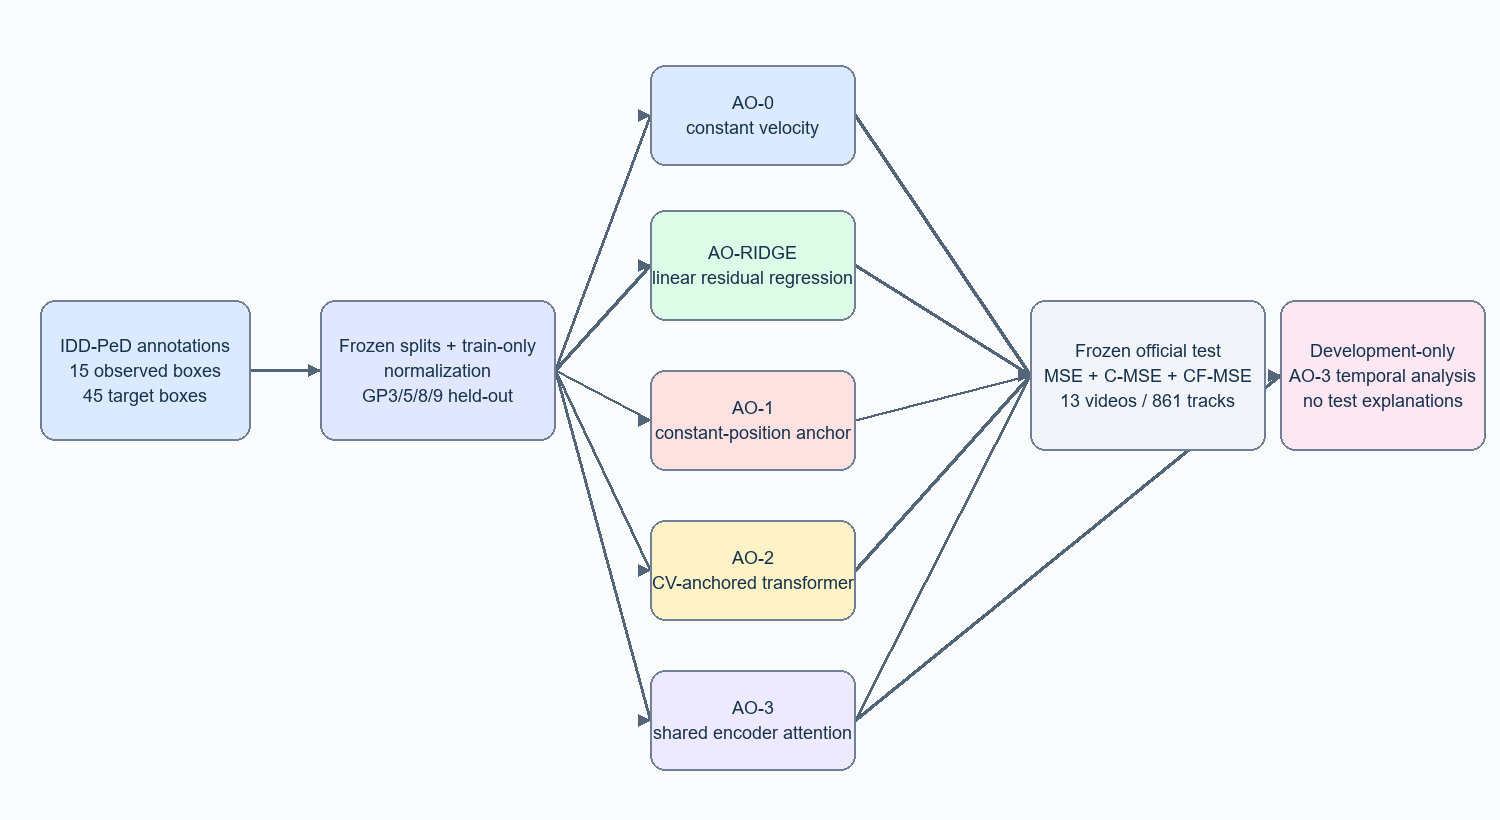
\includegraphics[width=.98\linewidth]{diagrams/overall_comparative_framework.png}\caption{Comparative study framework: the frozen annotation-only benchmark feeds the six evaluated models; CRAFT-inspired analysis is restricted to AO-3 development data.}\label{fig:framework}\end{figure}

\section{Related work}
Pedestrian forecasting spans datasets and models with substantially different input and output protocols. PIE established a large-scale pedestrian-intention and trajectory benchmark \citep{rasouli2019pie}. IDD-PeD provides pedestrian trajectory and intention prediction in unstructured traffic, with released MTN, BiTraP and SGNet baseline families \citep{bokkasam2025iddped}. MTN uses a multimodal transformer and may consume boxes, ego speed and optical flow \citep{yin2021mtn}; these richer inputs differ from our annotation-only setting. BiTraP models multimodal futures and SGNet uses goal-oriented forecasting; neither is numerically ranked against our models here because an identical split, deterministic output rule, coordinate representation and evaluation pipeline have not been established.

Social LSTM and Social GAN model interactions in pedestrian scenes \citep{alahi2016sociallstm,gupta2018socialgan}; Trajectron++, PECNet, AgentFormer address multimodal or map-aware forecasting under distinct representations and datasets \citep{salzmann2020trajectron,lee2020pecnet,yuan2021agentformer}. Their reported ADE/FDE or best-of-$K$ scores are not directly comparable to pooled box-coordinate MSE on IDD-PeD. CRAFT recursively factorizes nonnegative intermediate activations and uses Sobol sensitivity for image explanation \citep{fel2023craft}; our temporal adaptation has different representations and does not reproduce its image attribution or human evaluation. HIVE evaluates human interpretability with behavioral tasks such as distinction and agreement \citep{kim2022hive}; no participant study was conducted for this project.

\begin{table}[H]\centering\scriptsize
\caption{Published benchmark-relevant methods and compatibility. No external numerical scores are mixed into the direct ranking.}\begin{tabularx}{\linewidth}{p{2.0cm}p{2.15cm}p{4.1cm}X}
\toprule Method & Source & Published setting (high level) & Compatibility with this study \\
\midrule MTN & IDD-PeD / IJCAI & Transformer, potentially boxes plus ego speed/flow & Benchmark-relevant; full-input protocol differs \\
BiTraP & IDD-PeD & Multimodal trajectory baseline & Published setup/output selection must be aligned \\
SGNet & IDD-PeD & Goal-conditioned trajectory baseline & Split and forecast representation not matched \\
Social LSTM / Social GAN & PIE and related & Interaction-aware pedestrian forecasting & Different scenes, outputs and metrics \\
Trajectron++ / PECNet / AgentFormer & General trajectory prediction & Map, goal, multimodal or best-of-$K$ variants & Context and metrics differ; no numerical rank claim \\
\bottomrule\end{tabularx}\label{tab:published}
\end{table}

\section{Data, protocol and metrics}
The official test comprises 2,615 eligible windows across 13 videos and 861 $(video,track)$ clusters in GP3, GP5, GP8 and GP9. Every input is 15 consecutive absolute-pixel $xyxy$ boxes followed by the immediately adjacent 45 target boxes, under a 30-FPS convention. Eligible windows contain 60 consecutive valid frames and are sampled with stride 30; malformed, out-of-frame, non-positive-area or outside-annotation boxes break segments. No interpolation, image pixels, scene map, optical flow, ego speed, other-agent features, or future-derived input is used. All models use identical sample IDs/order and frozen train-only coordinate normalization where applicable.

The primary metric is pooled mean squared error over samples, 45 future frames, and four box coordinates:
\begin{equation}
\mathrm{MSE}=\frac{1}{N\cdot45\cdot4}\sum_{n=1}^{N}\sum_{t=1}^{45}\sum_{c\in\{x_1,y_1,x_2,y_2\}} (\hat y_{ntc}-y_{ntc})^2.
\end{equation}
Let $c_{nt}$ denote the centre of box $y_{nt}$. We define the center metrics as\begin{align}\mathrm{C\!-\!MSE}&=\frac{1}{45N}\sum_{n=1}^{N}\sum_{t=1}^{45}\|\hat c_{nt}-c_{nt}\|_2^2,\\\mathrm{CF\!-\!MSE}&=\frac{1}{N}\sum_{n=1}^{N}\|\hat c_{n,45}-c_{n,45}\|_2^2.\end{align} Horizon MSE is evaluated at steps 1, 15, 30 and 45. Per-video and per-track errors are computed first within unit; macro-video and macro-track summaries average those unit errors. The primary aggregate and secondary metrics are raw pixel units (MSE-family values in px$^2$).

\section{Models}
\subsection{Deterministic and classical baselines}
AO-0 extrapolates the last observed box using the coordinate-wise velocity $(x_{15}-x_{13})/2$ for each future step. AO-CP repeats the final observed box. AO-RIDGE constructs 64 features from the 60 normalized observed coordinates relative to the final box plus that final normalized box. Features are standardized using training data. Ridge predicts a 45-by-4 residual relative to a CV forecast in normalized coordinates; the fixed alpha is 100, selected on GP7 validation from the frozen grid. Its correction is added to the CV anchor before the same train-only inverse normalization. Thus the ridge result is validation-selected and remains descriptive on test.

\subsection{Annotation-only transformer ablations}
AO-1 uses a constant-position anchor; AO-2 and AO-3 use a CV anchor. Each model projects 4-D boxes to $d=32$, adds sinusoidal position encodings, applies a three-layer encoder with four-head self-attention and a ReLU FFN of dimensions $32\to128\to32$, then decodes 45 zero-box queries by three cross-attention/FFN layers against encoder memory. The decoder has no target self-attention. A $32\to4$ generator predicts a correction added to the selected anchor. In normalized coordinates the forecast is $\hat Y= A(X)+g_{\theta}(X)$, followed by the frozen inverse normalization for pixel scoring. Dropout is 0.1. AO-2 has 76,804 unique trainable parameters. AO-3, the compact candidate, ties the encoder self-attention module across all three encoder layers while leaving feedforward and normalization parameters independent; it has 68,356 trainable parameters. AO-2 was the predeclared primary neural accuracy candidate; AO-3 was the compact candidate. No roles were changed after test evaluation.

\begin{figure}[H]\centering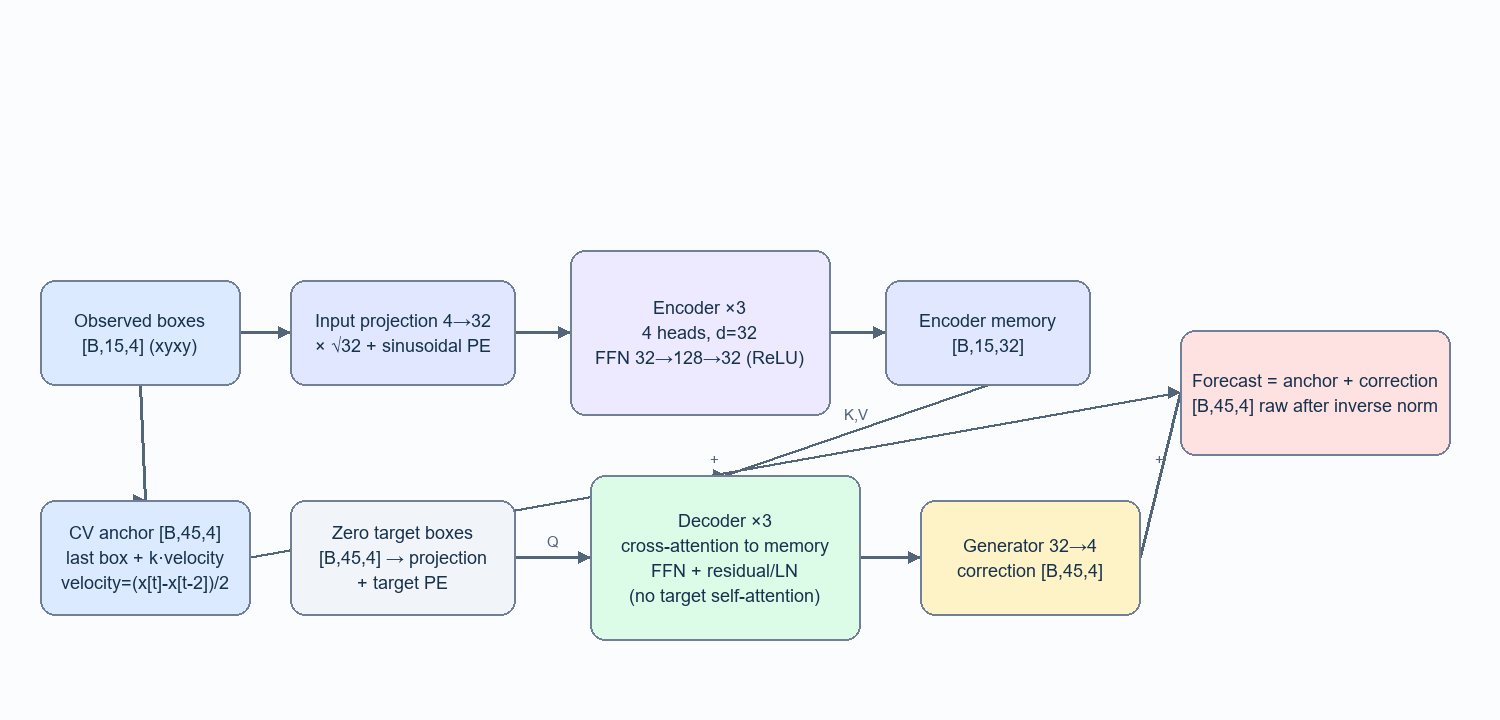
\includegraphics[width=.98\linewidth]{diagrams/cv_anchored_transformer.png}\caption{Implemented CV-anchored transformer paths and tensor dimensions. AO-1 changes the anchor to constant position.}\label{fig:transformer}\end{figure}
\begin{figure}[H]\centering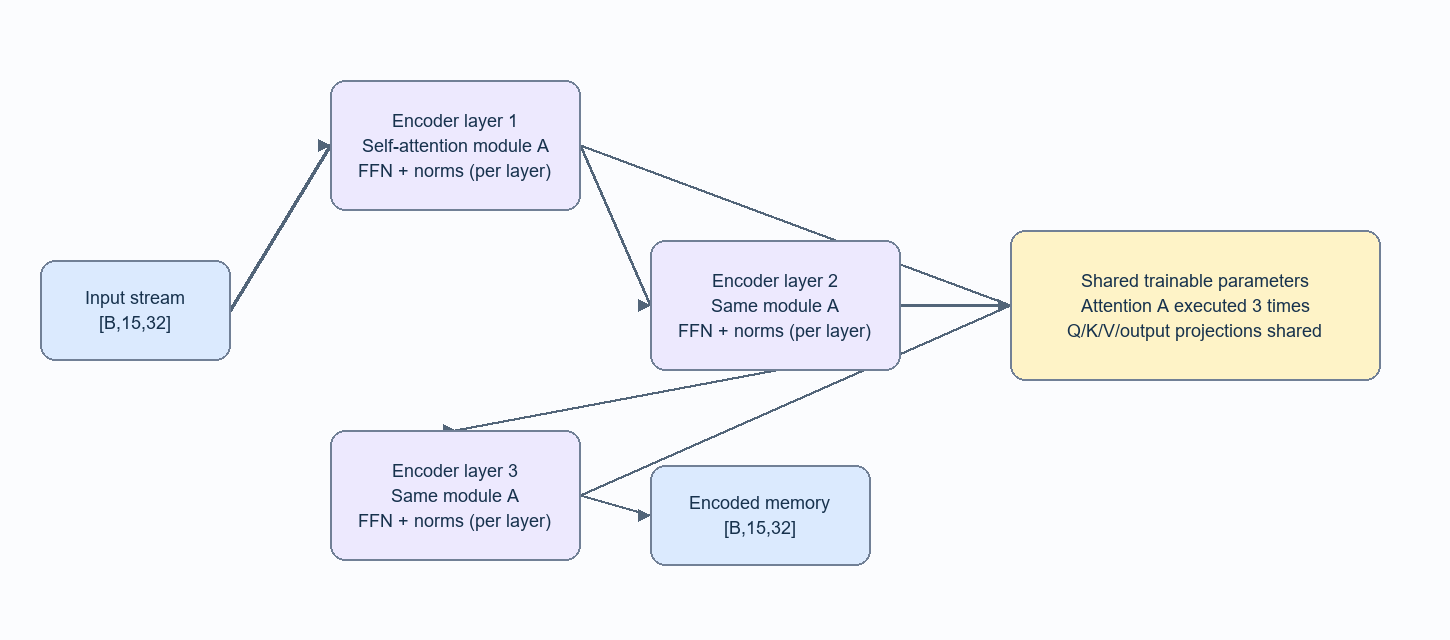
\includegraphics[width=.92\linewidth]{diagrams/satie_parameter_sharing.png}\caption{AO-3 shares the same encoder attention module at three executions; FFNs and layer norms remain layer-specific.}\label{fig:satie}\end{figure}
\begin{figure}[H]\centering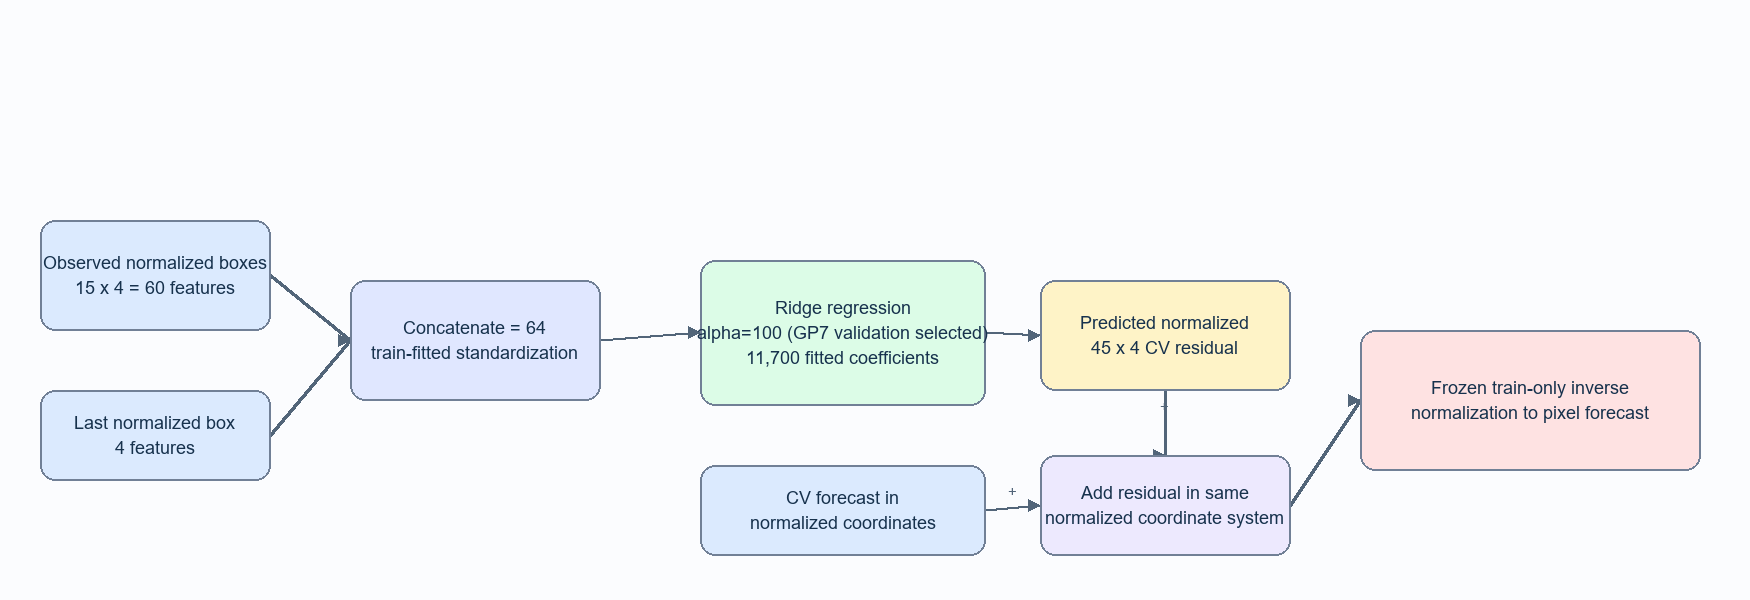
\includegraphics[width=.9\linewidth]{diagrams/ridge_residual_forecasting.png}\caption{AO-RIDGE learns normalized CV residuals and adds them before inverse normalization. The corrected path is unit-consistent.}\label{fig:ridge}\end{figure}

\section{Experimental design and statistical analysis}
The frozen checkpoint manifest contains five seeds for each neural AO model. Seeds are repeated training realizations on the same test sample membership, not independent test datasets. Planned paired seed differences are summarized with sample SD and 95\% $t$ intervals. A separate 10,000-replicate bootstrap resamples whole $(video,track)$ clusters; its intervals are conditional on the 861 observed clusters and answer a different sampling question. The seven planned comparisons and full procedure are in the frozen statistical analysis plan. No equivalence claim is made. The table reports complete five-seed means; the separate sensitivity analysis excluding resumed seed 20260928 is retained in the supporting report.

\section{Official-test results}
\begin{table}[H]\centering\small
\caption{Canonical corrected official-test results. Neural entries show mean $\pm$ sample SD across five seeds. Deterministic methods have one result.}\begin{tabular}{lrrrrrr}
\toprule Model & Runs & Parameters & MSE & C-MSE & CF-MSE & $\Delta$ vs CV \\
\midrule
AO-0 (CV) & 1 & 0 & 3997.237 & 6031.335 & 27599.699 & -- \\
AO-1 & 5 & 76804 & 8516.523 $\pm$ 1145.123 & 16072.016 & 57260.427 & +113.060\% \\
AO-2 & 5 & 76804 & 3975.058 $\pm$ 82.442 & 5907.203 & 25938.171 & -0.555\% \\
AO-3 & 5 & 68356 & 3962.073 $\pm$ 82.551 & 5877.412 & 25924.384 & -0.880\% \\
AO-RIDGE & 1 & 11700 & 2889.718 & 5244.799 & 24276.293 & -27.707\% \\
AO-CP & 1 & 0 & 11558.828 & 21746.627 & 80514.547 & +189.158\% \\
\bottomrule\end{tabular}\label{tab:official}
\end{table}

AO-RIDGE is the lowest-error frozen predictor. AO-2 and AO-3 are only 0.555\% and 0.880\% below CV by mean MSE. The CV-anchor transformer AO-2 improves on the constant-position residual ablation AO-1 by about 53.33\% in pooled MSE. This contrast supports the anchor choice within these models, not a general causal claim about physics.

\begin{table}[H]\centering\small
\caption{Individual official-test neural seed MSE (px$^2$). All seeds use the same fixed windows.}\begin{tabular}{r rrr}\toprule Seed & AO-1 & AO-2 & AO-3\\\midrule
20260928 & 10385.226 & 3992.012 & 3972.971\\
20260929 & 8501.335 & 3989.174 & 3954.972\\
20260930 & 7555.998 & 4005.926 & 3962.000\\
20260931 & 7605.475 & 4053.244 & 4076.577\\
20260932 & 8534.582 & 3834.936 & 3843.842\\\bottomrule\end{tabular}\label{tab:seeds}\end{table}

\begin{table}[H]\centering\small
\caption{Predeclared paired differences, first minus second. Neural comparisons use paired seed values and 95\% $t$ intervals. Ridge versus neural intervals use neural seed variability and are descriptive because ridge has one frozen fit.}\begin{tabular}{lrrr}\toprule Comparison & Mean difference & 95\% interval & Interpretation\\\midrule
AO-2 $-$ AO-1 & -4541.465 & [-5986.323, -3096.606] & Seed-paired\\
AO-2 $-$ AO-0 & -22.179 & [-124.544, 80.186] & Includes zero\\
AO-3 $-$ AO-0 & -35.165 & [-137.666, 67.336] & Includes zero\\
AO-3 $-$ AO-2 & -12.986 & [-48.337, 22.366] & Includes zero\\
AO-RIDGE $-$ AO-0 & -1107.519 & deterministic difference & Single outputs\\
AO-RIDGE $-$ AO-2 & -1085.340 & [-1187.705, -982.975] & Descriptive\\
AO-RIDGE $-$ AO-3 & -1072.354 & [-1174.855, -969.853] & Descriptive\\
\bottomrule\end{tabular}\label{tab:paired}\end{table}

\begin{table}[H]\centering\scriptsize
\caption{Track-cluster bootstrap intervals (10,000 replicates), first minus second; conditional on the observed $(video,track)$ clusters.}\begin{tabular}{p{5cm}p{7cm}}\toprule Comparison & 95\% bootstrap interval\\\midrule
AO-2 $-$ AO-1 & [-5820.981, -4287.765]\\
AO-2 $-$ AO-0 & [-515.327, -282.596]\\
AO-3 $-$ AO-0 & [-506.376, -279.113]\\
AO-3 $-$ AO-2 & [-16.097, -2.739]\\
AO-RIDGE $-$ AO-0 & [-1530.668, -1082.711]\\
AO-RIDGE $-$ AO-2 & [-1210.421, -632.147]\\
AO-RIDGE $-$ AO-3 & [-1206.444, -636.446]\\
\bottomrule\end{tabular}\label{tab:bootstrap}\end{table}

The cluster-bootstrap interval for AO-3 minus AO-2 was [-16.097,-2.739] MSE, whereas the seed-paired $t$ interval spans zero. These intervals are not contradictory: one summarizes variation across the observed track clusters conditional on the trained seed models, the other variation across five paired training seeds. Neither establishes broad population generalization. For AO-3 versus CV the cluster interval is [-506.376,-279.113], also conditional on observed clusters. The full bootstrap table is supplied.

\begin{table}[H]\centering\small
\caption{Macro performance across 13 videos and 861 track clusters. Values average each run's macro metric over available runs; neural rows average five seeds.}\begin{tabular}{lrr}\toprule Model & Macro-video MSE & Macro-track MSE\\\midrule
AO-0 & 3785.372 & 4975.977\\AO-1 & 8414.608 & 9553.045\\AO-2 & 3761.633 & 4540.468\\AO-3 & 3744.505 & 4530.801\\AO-RIDGE & 2747.340 & 3690.355\\AO-CP & 11265.549 & 15835.702\\\bottomrule\end{tabular}\label{tab:macro}\end{table}

Figure~\ref{fig:horizon} shows error growth through the forecast horizon. Per-video and per-track summaries reveal substantial heterogeneity, and the per-track distribution is long-tailed. These are descriptive secondary views; the primary frozen ranking remains pooled MSE.
\begin{figure}[H]\centering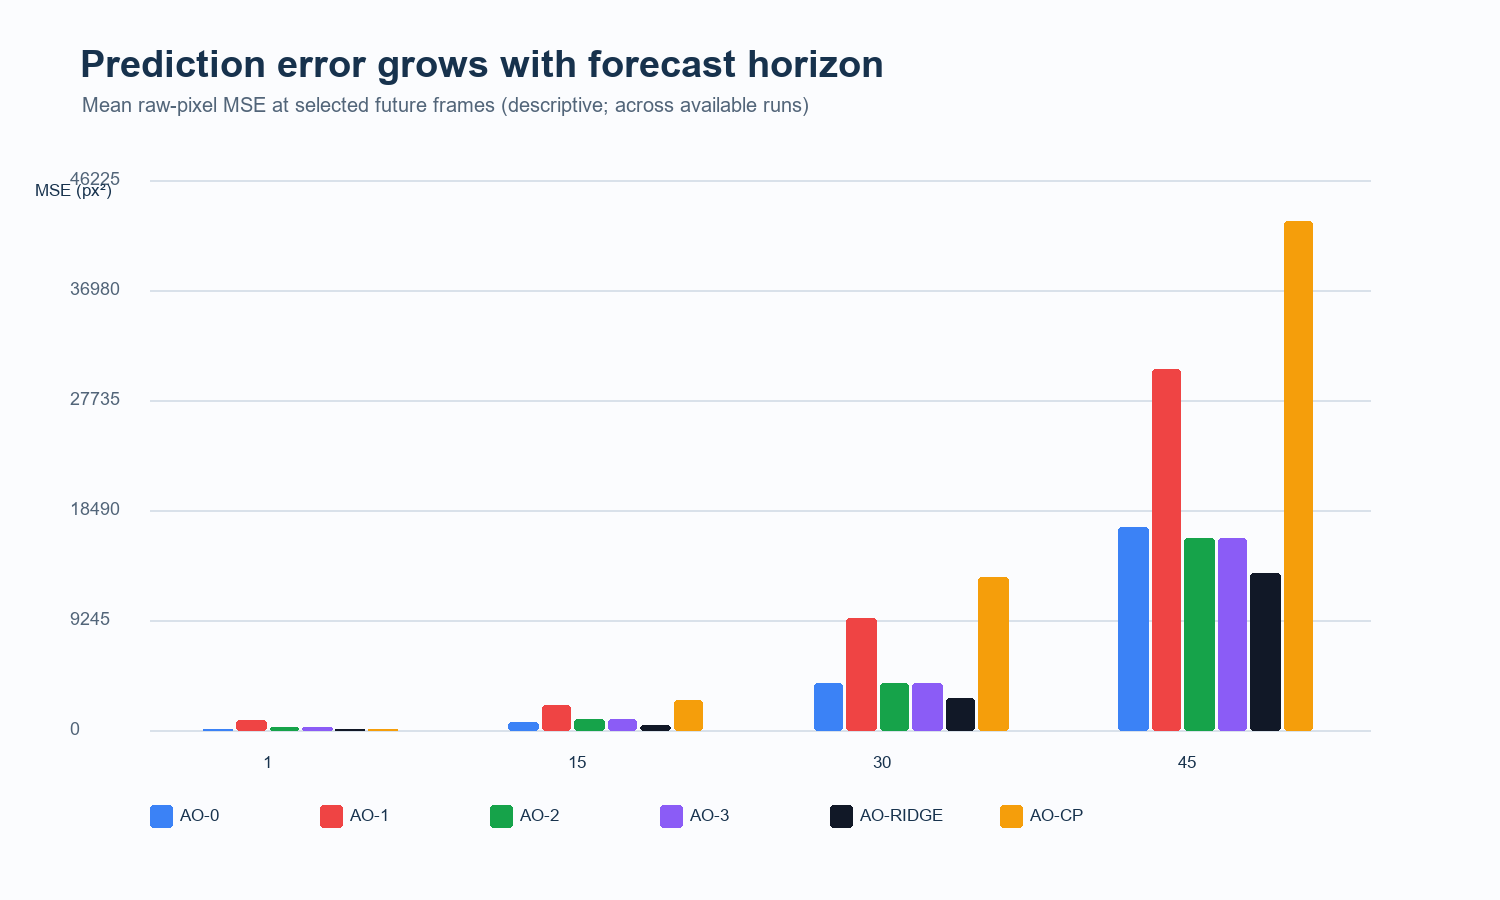
\includegraphics[width=.95\linewidth]{figures/horizon_mse.png}\caption{Raw-pixel MSE at four forecast steps, aggregated over available model runs.}\label{fig:horizon}\end{figure}
\begin{figure}[H]\centering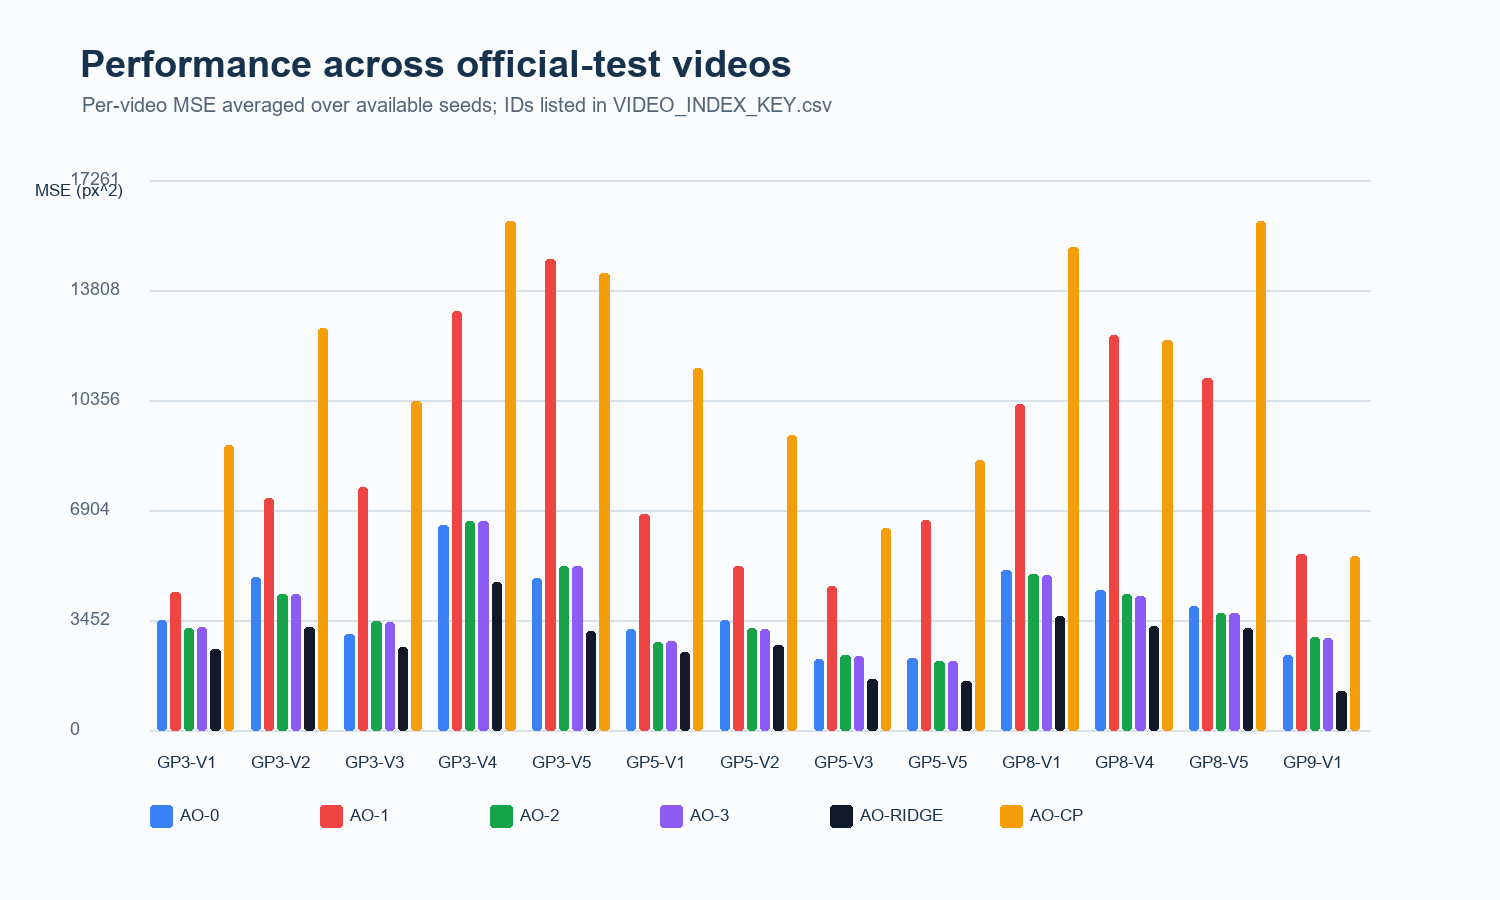
\includegraphics[width=.98\linewidth]{figures/per_video_mse.png}\caption{Per-video MSE averaged across available runs. Every listed video is part of the frozen official-test membership.}\label{fig:pervideo}\end{figure}
\begin{figure}[H]\centering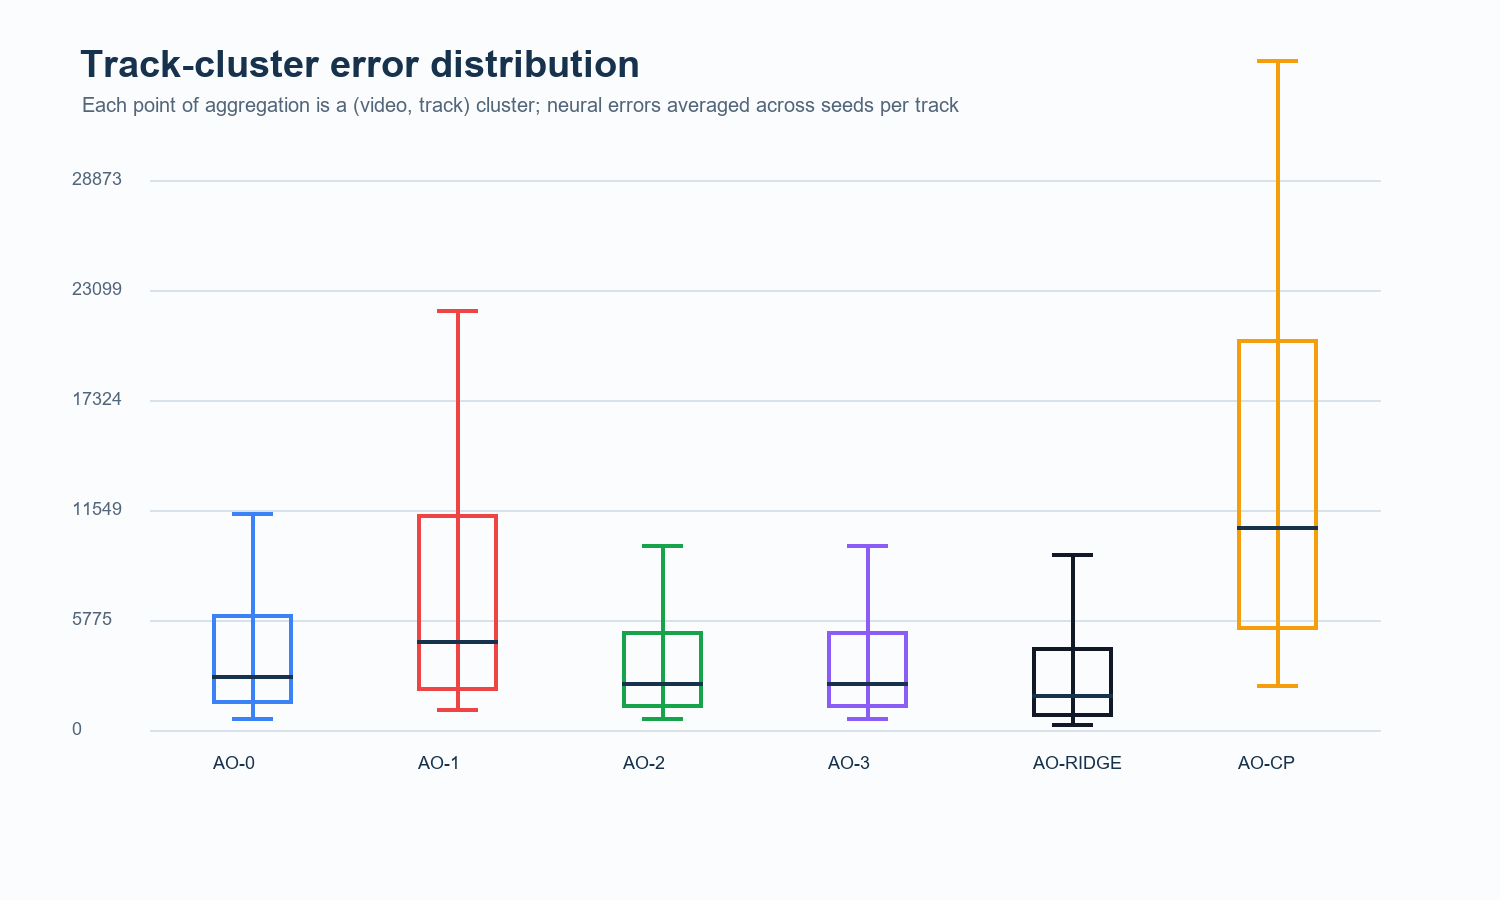
\includegraphics[width=.82\linewidth]{figures/per_track_distribution.png}\caption{Track-cluster error distribution; neural values are averaged over seed values within each cluster. Whiskers show the 10th--90th percentiles.}\label{fig:pertrack}\end{figure}
\begin{figure}[H]\centering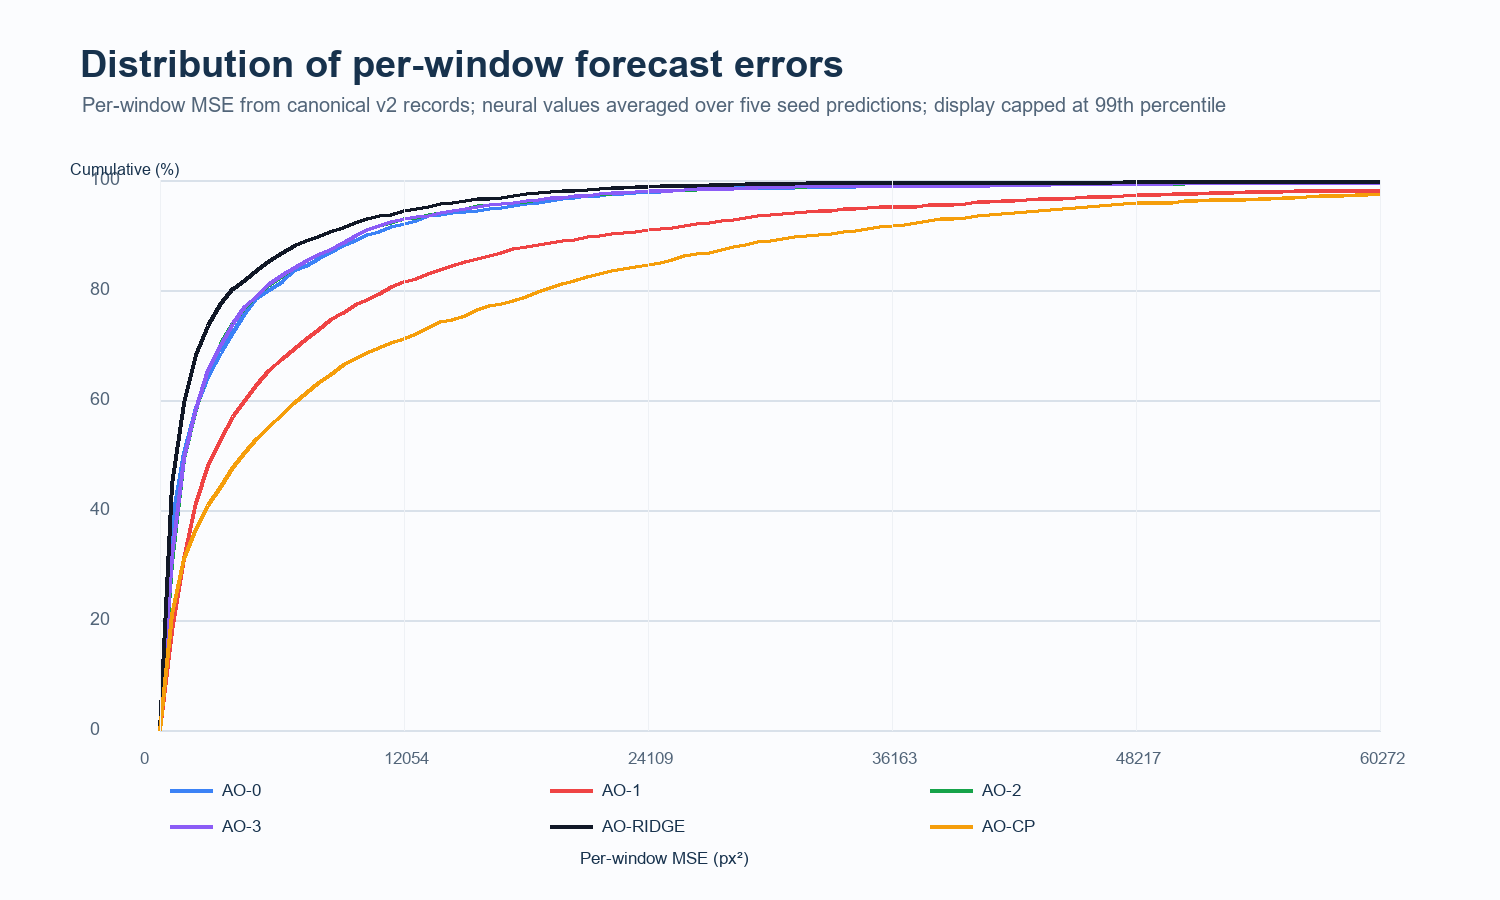
\includegraphics[width=.82\linewidth]{figures/per_window_error_ecdf.png}\caption{Empirical CDF of per-window MSE. For neural models, each sample's errors are averaged across the five seeds; the plotted x-range ends at the pooled 99th percentile.}\label{fig:ecdf}\end{figure}
\begin{figure}[H]\centering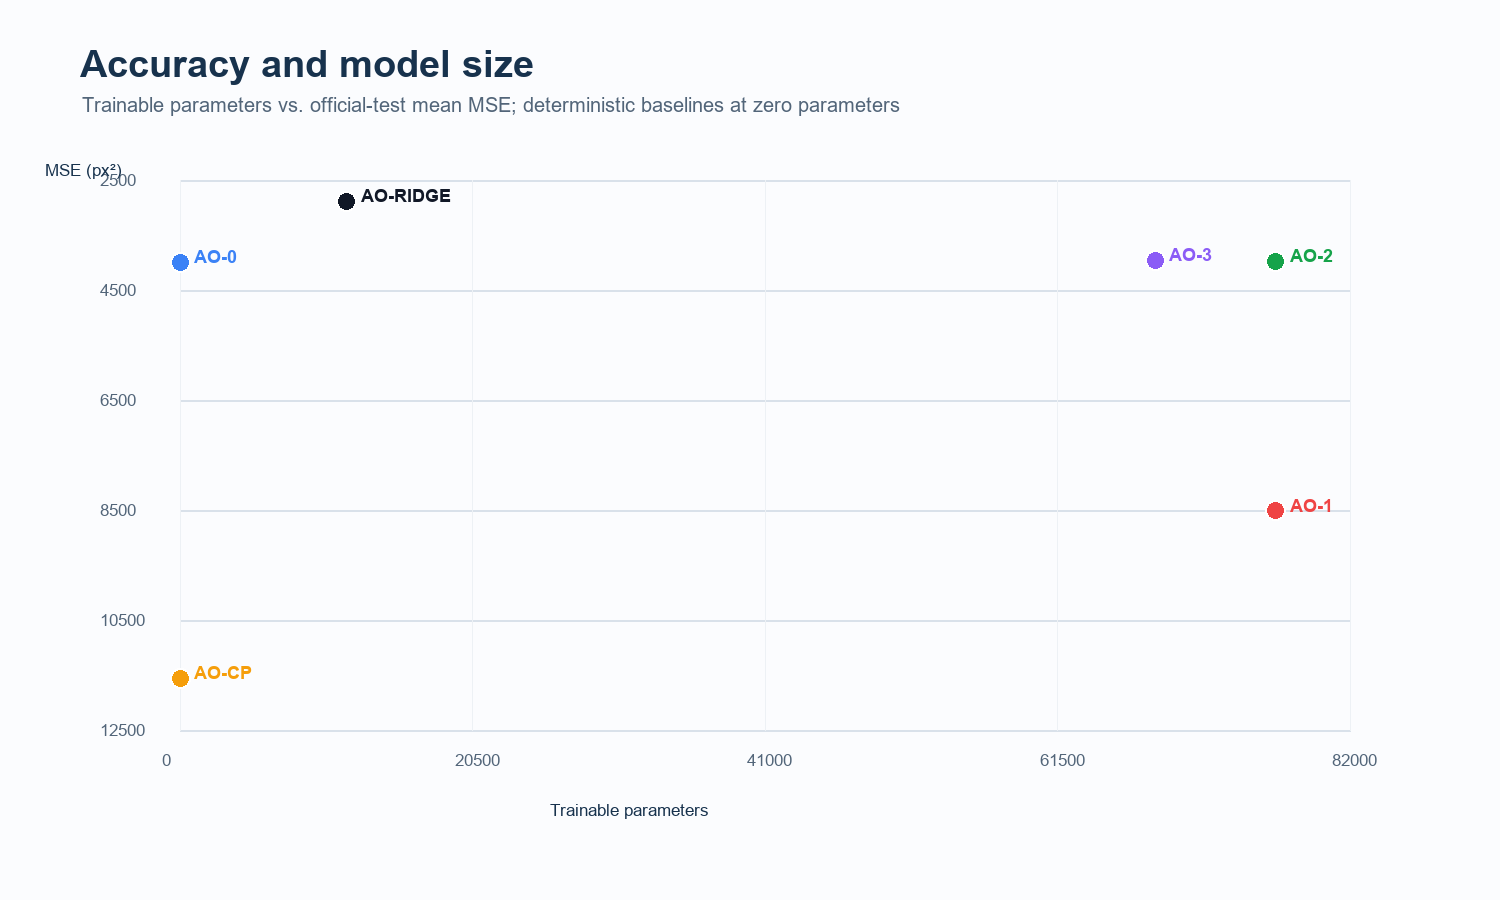
\includegraphics[width=.72\linewidth]{figures/parameter_accuracy.png}\caption{Parameter count versus primary official-test MSE. The deterministic baselines have no trainable parameters.}\label{fig:params}\end{figure}

\subsection{Ridge correction and artifact integrity}
The initial v1 evaluator mixed a normalized-coordinate ridge residual with a raw-pixel CV forecast, producing an invalid unit combination before scoring. In v2, CV is formed in normalized coordinates, the frozen normalized residual is added there, and the same train-only inverse normalization is applied once. The change altered only the deterministic AO-RIDGE seed 20260928 record (3,986.643 to 2,889.718 MSE); video membership, annotation hashes, sample order, neural results, checkpoint hashes and alpha 100 were unchanged. This was a coordinate-consistency bug fix, not test-driven tuning. The v2 bundle and v3 derived summaries are canonical; v1 remains preserved as superseded history.

\section{Computational efficiency}
The matched CPU benchmark used an Intel i5-8365U, four threads, 50 warm-ups and 500 timed iterations. AO-2 median latency was 99.049 ms at batch 1 and 114.574 ms at batch 8; AO-3 was 49.395 and 102.235 ms. This single-machine benchmark is not a broad hardware comparison. Official-test wall-clock inference time was not recorded and is not reported. SATIE reduces unique trainable parameters by 8,448 (11.0\%) relative to AO-2, with no seed-level conclusive MSE improvement.

\section{Qualitative analysis and human-centered evaluation readiness}
The corrected Phase 6B bundle stores per-window errors and sample identifiers but not observed, future, or predicted box-coordinate arrays. Consequently, an honest official-test trajectory overlay or representative predicted success/failure trajectory figure cannot be made from the saved official artifacts. Producing those coordinates would require rerunning inference, which is outside this frozen manuscript phase. The metrics-based horizon, video, track, error-distribution and parameter figures above are reproducible from existing outputs. Historical E1 attention/overlay materials belong to a different model/input configuration and are not presented as AO-2/AO-3 evidence.

We prepared a HIVE-style study protocol based on distinction and agreement tasks, neutral blinded forecasts, counterbalanced candidate order and secondary comprehension/confidence questions. This is design-only. No participants were recruited and no responses exist. The historical E1 sample bank is unsuitable as the final AO comparison because it represents a different model family, comes from a single video and has presentation confounds. New AO stimuli require saved coordinate predictions plus video-data permissions, anonymization, institutional ethics review, informed consent and preregistration. HIVE outcomes are not empirical results in this paper.

\section{CRAFT-inspired temporal concept analysis}
We analyzed the frozen AO-3 seed-20260928 model using development data only. Genuine nonnegative ReLU FFN activations were saved for 988 training and 432 GP7 validation windows, with shape $[N,15,128]$. An exploratory rank-4 NMF bank fit in original activation coordinates produced relative Frobenius errors 0.175750 on training and 0.371239 on validation; matched factor cosine stability was 1.000000 and the full refit converged in 62 iterations. Identity intervention output error was exactly zero; reconstruction intervention relative output deviation was 0.0027753 on the Stage 2B sampled check.

Three of four selected parent concepts passed the recursive numerical screen; C1 reached its 200-iteration cap with convergence warnings. Three descriptive associations met the fixed threshold: C1 with mean observed velocity ($\rho=-0.519$), C1 with observed acceleration ($\rho=-0.386$), and C3 with mean velocity ($\rho=0.304$). Because the windows overlap and are clustered, the window-level p-values are descriptive. No factors receive semantic labels.

The Stage 3 Sobol analysis used 32 GP7 windows and four explicitly defined scalar outputs: final predicted center $x$, final center $y$, final displacement norm, and CV-correction energy. All four sensitivity estimates converged under the declared rule. Within the selected FFN branch and independent uniform amplitude intervention, C2 dominated center coordinates and correction energy; C4 dominated displacement norm. This local branch-relative sensitivity must not be read as global model importance. Seven of eight insertion/deletion screens passed, with displacement-norm deletion failing. The chosen activation branch had limited effects on center/displacement summaries; small absolute effects can inflate normalized fidelity AUCs. The experiment is exploratory, factors were not semantically validated, and the sensitivity sample was small.

This is a CRAFT-inspired adaptation, not a faithful CRAFT reproduction: there are no implicit-differentiation attribution maps, validated semantic concepts, or human utility experiments. The reference method was developed for image concepts and includes distinct visualization and fidelity procedures. Our temporal coefficients and interventions do not demonstrate spatial image explanations.
\begin{figure}[H]\centering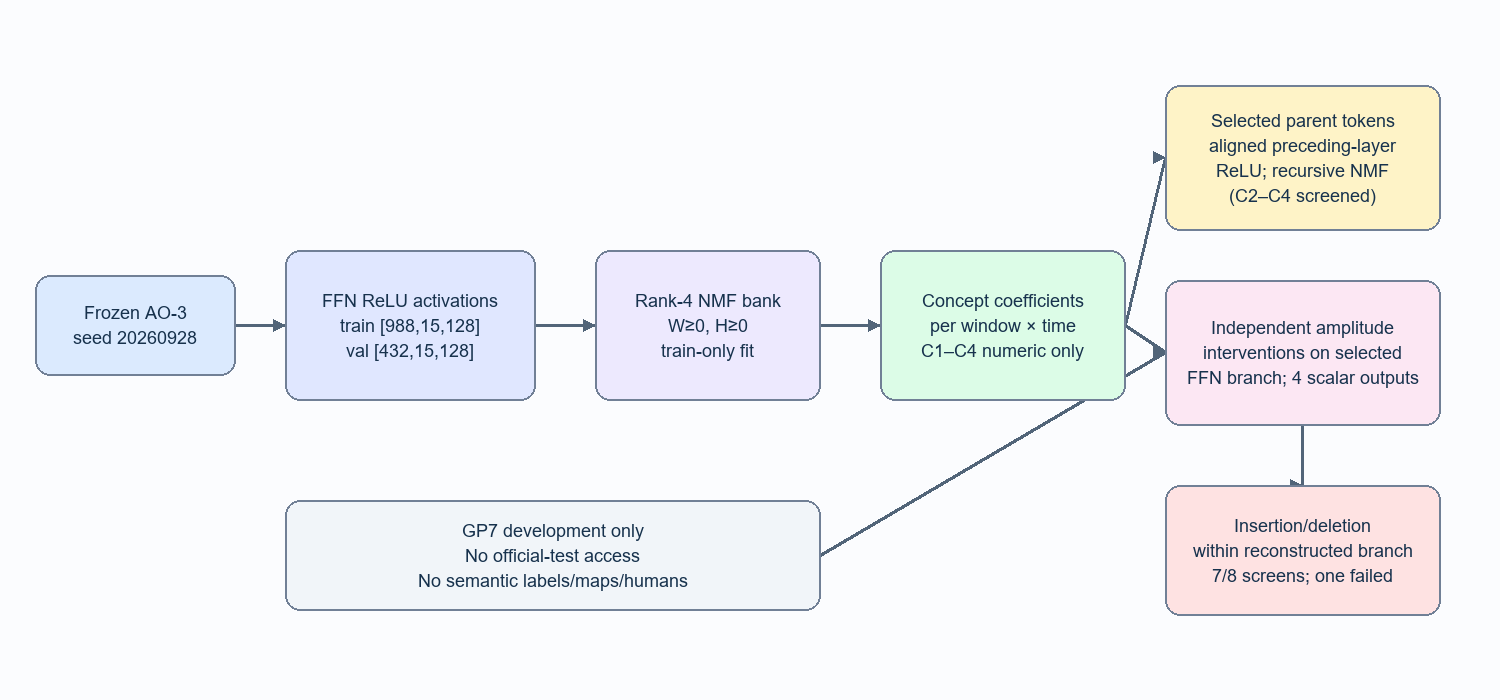
\includegraphics[width=.98\linewidth]{diagrams/craft_temporal_concepts.png}\caption{Temporal adaptation path: training-derived nonnegative factors and held-out coefficients feed bounded recursive, Sobol and fidelity probes on development data only.}\label{fig:craftworkflow}\end{figure}
\begin{figure}[H]\centering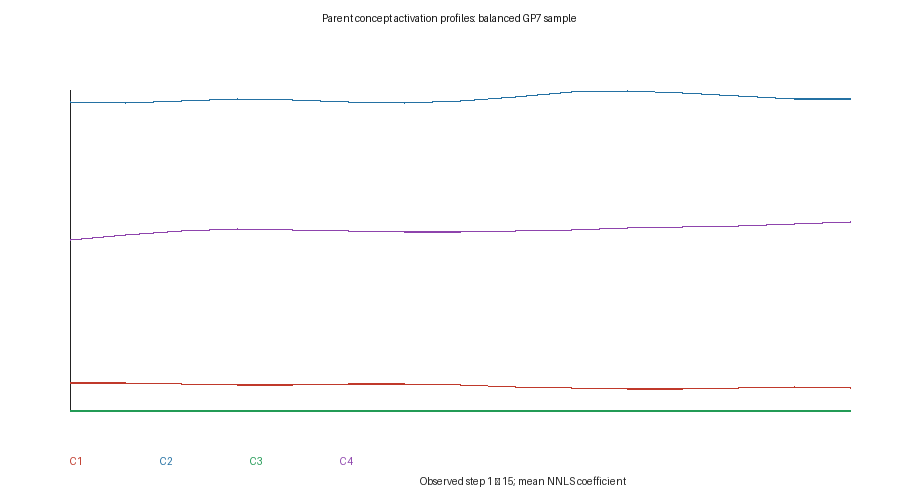
\includegraphics[width=.8\linewidth]{figures/craft/PARENT_CONCEPT_PROFILES.png}\caption{AO-3 rank-4 temporal coefficient profiles from the verified development-only CRAFT-inspired analysis. Numeric labels are retained.}\end{figure}
\begin{figure}[H]\centering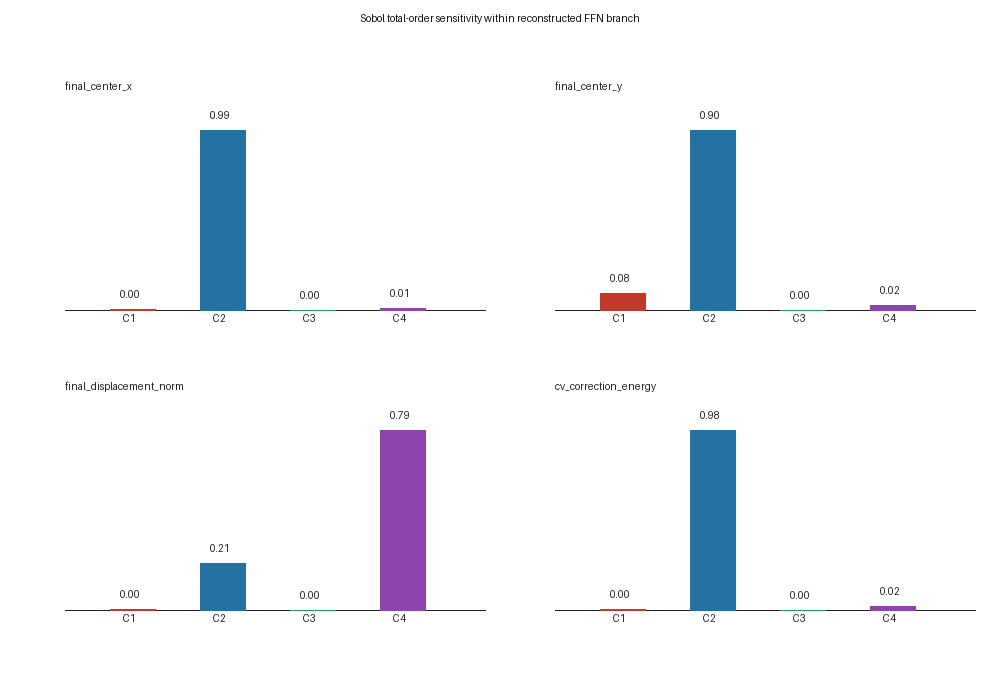
\includegraphics[width=.86\linewidth]{figures/craft/SOBOL_IMPORTANCE.png}\caption{Branch-relative Sobol sensitivities for four predefined scalar outputs; not global model importance.}\end{figure}
\begin{figure}[H]\centering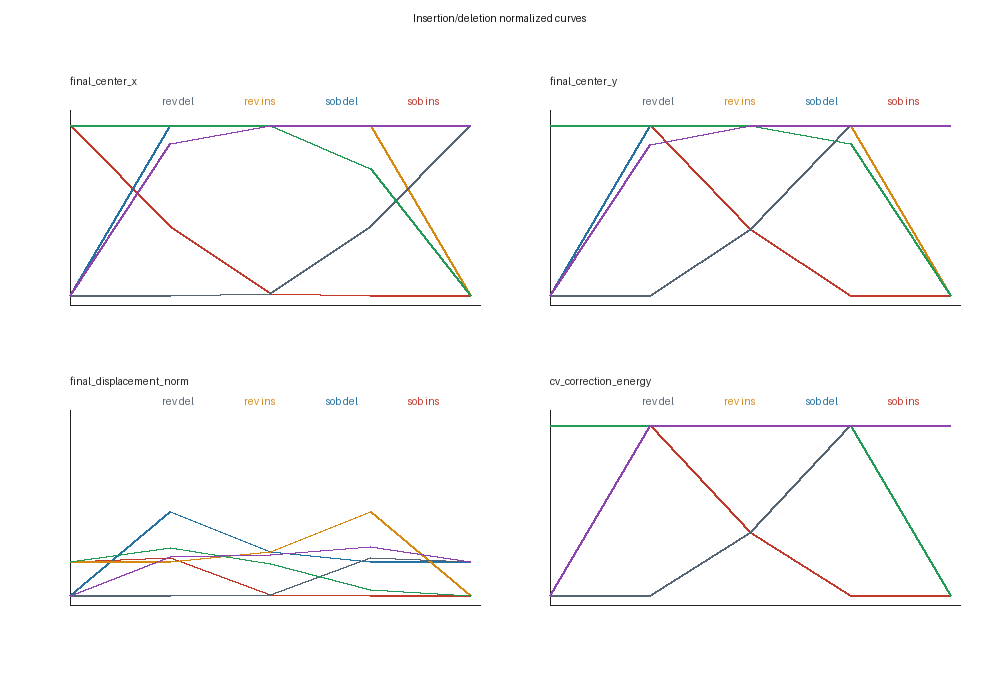
\includegraphics[width=.86\linewidth]{figures/craft/INSERTION_DELETION_FIDELITY.png}\caption{Insertion/deletion fidelity screens, including the failed displacement-norm deletion screen.}\end{figure}

\section{Architecture naming and interpretation}
AO-3 can retain ``PACE-Net'' as a project label only if expanded as ``Physics-Anchored Compact Encoding Network'' and defined narrowly: ``physics-anchored'' refers solely to adding a constant-velocity kinematic forecast, not learned physical laws or constrained dynamics; ``compact encoding'' refers to tied encoder self-attention weights. The paper uses AO-3 as its primary technical identifier to avoid overstating novelty. No four-module naming scheme is proposed because no such four modules exist in the frozen implementation. Historical SAGE, MASC and ROUTE experiments are exploratory context analyses and are not modules in the final annotation-only predictor; they did not establish consistent gains in the final study.

\section{Limitations}
The conclusions condition on one dataset, a fixed official-test membership of 13 videos, and an annotation-only 15/45 protocol. Overlapping windows are dependent. Five seeds characterize initialization/training variability but do not create independent test samples. Cluster bootstrap intervals condition on the observed clusters, and video-level generalization remains uncertain. Ridge alpha was selected on two GP7 validation videos, so ridge's test result is not a fully untouched model-selection outcome, although test data did not select alpha. The fixed CV rule may be sensitive to annotation jitter and camera geometry. The official prediction coordinate arrays are absent from the saved bundle, preventing forecast trace illustrations. The CRAFT-inspired analysis is exploratory and branch-specific; its factor labels, causal meaning and generality are not established. No human evaluation, safety assessment or deployment study was performed. Published methods use incompatible inputs, datasets, coordinate systems and metrics, precluding state-of-the-art ranking.

\section{Conclusion}
On the frozen annotation-only IDD-PeD test protocol, the validation-selected ridge residual model achieved the lowest observed MSE and improved on CV by 27.707\%. The two CV-anchored neural candidates were close to the strong CV baseline, with paired seed-level intervals including zero. Sharing encoder attention reduced AO-3 parameters by 11.0\%, but the results do not establish a predictive advantage over AO-2. The bounded CRAFT-inspired investigation yields reproducible temporal factorization and local sensitivity diagnostics, alongside explicit convergence and fidelity failures; it does not validate semantic concepts or human utility. These findings support protocol-matched classical baselines, transparent uncertainty, and cautious claims in unstructured-traffic trajectory forecasting.

\bibliographystyle{plainnat}
\bibliography{references}
\end{document}



